\documentclass[tikz,border=2pt]{standalone}
\usepackage{amsmath}
\usepackage{pgfplots}
\pgfplotsset{compat=1.18}
\usetikzlibrary{arrows.meta}
\begin{document}
% Annotated print-out of the six-row emissions tibble printed with n = 3:
% size line (6 x 5), column names, column types, numbered rows, closing line "3 more rows".
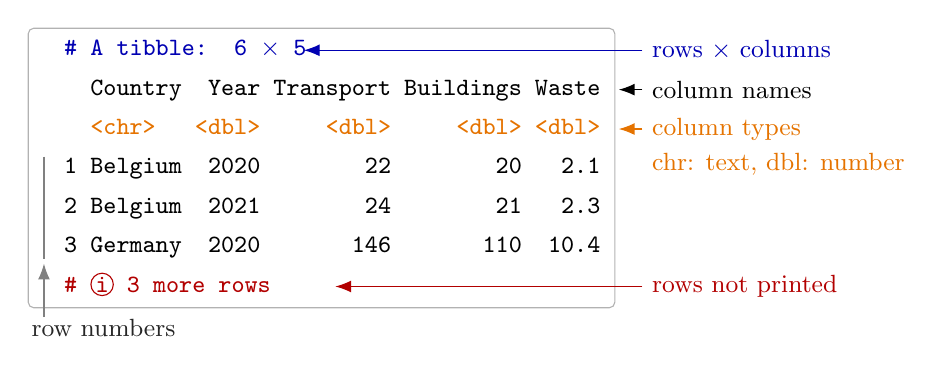
\begin{tikzpicture}[font=\small, >={Latex[length=2mm]},
  line/.style={anchor=base west, inner sep=0pt, font=\small\ttfamily},
  note/.style={anchor=west, align=left}]
  \def\dy{0.5}
  % the printed lines
  \node[line, blue!70!black] (l1) at (0,0) {\# A tibble: 6 $\times$ 5};
  \node[line] (l2) at (0,-1*\dy) {\ \ Country\ \ Year Transport Buildings Waste};
  \node[line, orange!90!black] (l3) at (0,-2*\dy) {\ \ <chr>\ \ \ <dbl>\ \ \ \ \ <dbl>\ \ \ \ \ <dbl> <dbl>};
  \node[line] (l4) at (0,-3*\dy) {1 Belgium\ \ 2020\ \ \ \ \ \ \ \ 22\ \ \ \ \ \ \ \ 20\ \ \ 2.1};
  \node[line] (l5) at (0,-4*\dy) {2 Belgium\ \ 2021\ \ \ \ \ \ \ \ 24\ \ \ \ \ \ \ \ 21\ \ \ 2.3};
  \node[line] (l6) at (0,-5*\dy) {3 Germany\ \ 2020\ \ \ \ \ \ \ 146\ \ \ \ \ \ \ 110\ \ 10.4};
  \node[line, red!70!black] (l7) at (0,-6*\dy) {\# \tikz[baseline=(c.base)]\node(c)[circle, draw, inner sep=0.3pt, font=\small\ttfamily]{i}; 3 more rows};
  % frame around the print-out
  \draw[gray!60, rounded corners=2pt] (-0.45,0.35) rectangle (7.0,-6*\dy-0.2);
  % row numbers
  \draw[gray, thick] (-0.25,-3*\dy+0.22) -- (-0.25,-5*\dy-0.08);
  \draw[->, gray] (-0.25,-6*\dy-0.32) -- (-0.25,-5*\dy-0.14);
  \node[gray!30!black, anchor=north west, inner sep=1pt] at (-0.45,-6*\dy-0.3) {row numbers};
  % annotations on the right
  \def\nx{7.35}
  \draw[->, blue!70!black] (\nx,0.07) -- (\nx-0.3,0.07) -- (3.05,0.07);
  \node[note, blue!70!black] at (\nx,0.07) {rows $\times$ columns};
  \node[note] at (\nx,-1*\dy+0.07) {column names};
  \draw[->] (\nx,-1*\dy+0.07) -- (7.05,-1*\dy+0.07);
  \node[note, orange!90!black] at (\nx,-2*\dy+0.07) {column types};
  \draw[->, orange!90!black] (\nx,-2*\dy+0.07) -- (7.05,-2*\dy+0.07);
  \node[note, orange!90!black] at (\nx,-2*\dy-0.38) {chr: text, dbl: number};
  \node[note, red!70!black] at (\nx,-6*\dy+0.07) {rows not printed};
  \draw[->, red!70!black] (\nx,-6*\dy+0.07) -- (3.45,-6*\dy+0.07);
\end{tikzpicture}
\end{document}
